\section{Film preparation}
\label{sec:FilmProd}

In the following section the film production is explained.

\subsection*{Substrate and solution production}

The following section explains how the sample substrate is produced.

As substrate glass slides are used. We cut those slides in rectangles of the dimension \SI[]{15}{mm} x \SI[]{25}{mm}. Afterwards the
glass slides were cleaned in the following liquids in the ultrasonic bath for 10 minutes and dried afterwards with nitrogen:

\begin{enumerate}
    \item Aqueous Alconox solution $0.16\,\frac{\mathrm{g}}{\mathrm{ml}}$
    \item Deionised water
    \item 2-Propanol
\end{enumerate}

The chlorobenzene and polystyrene solution used is prepared from a solution of \SI{300}{\milli\gram\per\milli\liter} by dilution. 
We produce approximately \SI{250}{\micro\liter} of solutions with the concentrations \SI{300}{\milli\gram\per\milli\liter}, \SI{250}{\milli\gram\per\milli\liter}, \SI{200}{\milli\gram\per\milli\liter},
\SI{150}{\milli\gram\per\milli\liter}, \SI{100}{\milli\gram\per\milli\liter}, \SI{50}{\milli\gram\per\milli\liter}, \SI{25}{\milli\gram\per\milli\liter} and \SI{1}{\milli\gram\per\milli\liter}.

\subsection*{Spincoating}

The films are produced using static spincoating.
In this method the solution is placed on the substrate. The spincoater is starting to spin the substrate. The centrifugal forces drive the solution away from the substrate.
This process enables the production of very homogeneous and thin layers.  

\begin{figure}[ht]
    \centering
    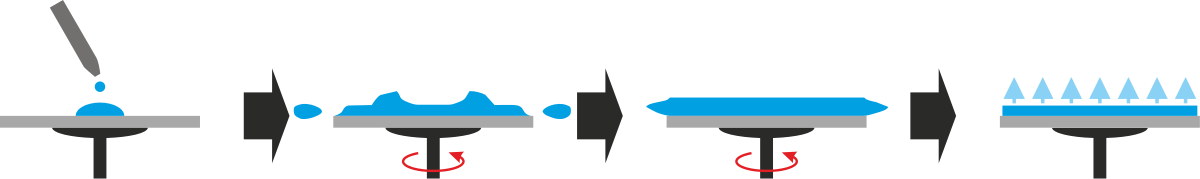
\includegraphics[width = \linewidth]{Bilder/Grundlagen/Spincoating.png}
    \caption[Graphical representation of the spincoating]{Graphical representation of the spincoating. From left to right, solution is placed in the substrate, the the coater spins and distributes the solution on the substrate. Afterwards the substrate drys.  From \textit{Stefan Reich \protect\footnotemark} }
    \label{fig:Spincoat}
\end{figure}

\footnotetext{(\url{https://commons.wikimedia.org/wiki/File:Spincoating.svg}), „Spincoating“, \url{https://creativecommons.org/publicdomain/zero/1.0/legalcode} }

We spincoat \SI{100}{\micro\litre} of the polymer solution onto the substrate.
The films for rotations dependence measurement were coated from a solution of \SI{100}{\milli\gram\per\milli\liter} at rotation rates of
\SI{500}{rpm}, \SI{750}{rpm}, \SI{1000}{rpm}, \SI{2000}{rpm}, \SI{3000}{rpm}, \SI{4000}{rpm} and \SI{5000}{rpm} for \SI{30}{\second}. This was done by \textit{Fabian Eller}.
Afterwards, a set of films is coated all with \SI{1000}{rpm} for \SI[]{90}{\second} but with all the above mentioned concentrations.